\documentclass[journal, a4paper]{IEEEtran}

% some very useful LaTeX packages include:

%\usepackage{cite}      % Written by Donald Arseneau
                        % V1.6 and later of IEEEtran pre-defines the format
                        % of the cite.sty package \cite{} output to follow
                        % that of IEEE. Loading the cite package will
                        % result in citation numbers being automatically
                        % sorted and properly "ranged". i.e.,
                        % [1], [9], [2], [7], [5], [6]
                        % (without using cite.sty)
                        % will become:
                        % [1], [2], [5]--[7], [9] (using cite.sty)
                        % cite.sty's \cite will automatically add leading
                        % space, if needed. Use cite.sty's noadjust option
                        % (cite.sty V3.8 and later) if you want to turn this
                        % off. cite.sty is already installed on most LaTeX
                        % systems. The latest version can be obtained at:
                        % http://www.ctan.org/tex-archive/macros/latex/contrib/supported/cite/

\usepackage{graphicx}   % Written by David Carlisle and Sebastian Rahtz
                        % Required if you want graphics, photos, etc.
                        % graphicx.sty is already installed on most LaTeX
                        % systems. The latest version and documentation can
                        % be obtained at:
                        % http://www.ctan.org/tex-archive/macros/latex/required/graphics/
                        % Another good source of documentation is "Using
                        % Imported Graphics in LaTeX2e" by Keith Reckdahl
                        % which can be found as esplatex.ps and epslatex.pdf
                        % at: http://www.ctan.org/tex-archive/info/

%\usepackage{psfrag}    % Written by Craig Barratt, Michael C. Grant,
                        % and David Carlisle
                        % This package allows you to substitute LaTeX
                        % commands for text in imported EPS graphic files.
                        % In this way, LaTeX symbols can be placed into
                        % graphics that have been generated by other
                        % applications. You must use latex->dvips->ps2pdf
                        % workflow (not direct pdf output from pdflatex) if
                        % you wish to use this capability because it works
                        % via some PostScript tricks. Alternatively, the
                        % graphics could be processed as separate files via
                        % psfrag and dvips, then converted to PDF for
                        % inclusion in the main file which uses pdflatex.
                        % Docs are in "The PSfrag System" by Michael C. Grant
                        % and David Carlisle. There is also some information
                        % about using psfrag in "Using Imported Graphics in
                        % LaTeX2e" by Keith Reckdahl which documents the
                        % graphicx package (see above). The psfrag package
                        % and documentation can be obtained at:
                        % http://www.ctan.org/tex-archive/macros/latex/contrib/supported/psfrag/

%\usepackage{subfigure} % Written by Steven Douglas Cochran
                        % This package makes it easy to put subfigures
                        % in your figures. i.e., "figure 1a and 1b"
                        % Docs are in "Using Imported Graphics in LaTeX2e"
                        % by Keith Reckdahl which also documents the graphicx
                        % package (see above). subfigure.sty is already
                        % installed on most LaTeX systems. The latest version
                        % and documentation can be obtained at:
                        % http://www.ctan.org/tex-archive/macros/latex/contrib/supported/subfigure/

\usepackage{url}        % Written by Donald Arseneau
                        % Provides better support for handling and breaking
                        % URLs. url.sty is already installed on most LaTeX
                        % systems. The latest version can be obtained at:
                        % http://www.ctan.org/tex-archive/macros/latex/contrib/other/misc/
                        % Read the url.sty source comments for usage information.

%\usepackage{stfloats}  % Written by Sigitas Tolusis
                        % Gives LaTeX2e the ability to do double column
                        % floats at the bottom of the page as well as the top.
                        % (e.g., "\begin{figure*}[!b]" is not normally
                        % possible in LaTeX2e). This is an invasive package
                        % which rewrites many portions of the LaTeX2e output
                        % routines. It may not work with other packages that
                        % modify the LaTeX2e output routine and/or with other
                        % versions of LaTeX. The latest version and
                        % documentation can be obtained at:
                        % http://www.ctan.org/tex-archive/macros/latex/contrib/supported/sttools/
                        % Documentation is contained in the stfloats.sty
                        % comments as well as in the presfull.pdf file.
                        % Do not use the stfloats baselinefloat ability as
                        % IEEE does not allow \baselineskip to stretch.
                        % Authors submitting work to the IEEE should note
                        % that IEEE rarely uses double column equations and
                        % that authors should try to avoid such use.
                        % Do not be tempted to use the cuted.sty or
                        % midfloat.sty package (by the same author) as IEEE
                        % does not format its papers in such ways.

\usepackage{amsmath}    % From the American Mathematical Society
                        % A popular package that provides many helpful commands
                        % for dealing with mathematics. Note that the AMSmath
                        % package sets \interdisplaylinepenalty to 10000 thus
                        % preventing page breaks from occurring within multiline
                        % equations. Use:
%\interdisplaylinepenalty=2500
                        % after loading amsmath to restore such page breaks
                        % as IEEEtran.cls normally does. amsmath.sty is already
                        % installed on most LaTeX systems. The latest version
                        % and documentation can be obtained at:
                        % http://www.ctan.org/tex-archive/macros/latex/required/amslatex/math/



% Other popular packages for formatting tables and equations include:

%\usepackage{array}
% Frank Mittelbach's and David Carlisle's array.sty which improves the
% LaTeX2e array and tabular environments to provide better appearances and
% additional user controls. array.sty is already installed on most systems.
% The latest version and documentation can be obtained at:
% http://www.ctan.org/tex-archive/macros/latex/required/tools/

% V1.6 of IEEEtran contains the IEEEeqnarray family of commands that can
% be used to generate multiline equations as well as matrices, tables, etc.

% Also of notable interest:
% Scott Pakin's eqparbox package for creating (automatically sized) equal
% width boxes. Available:
% http://www.ctan.org/tex-archive/macros/latex/contrib/supported/eqparbox/

% *** Do not adjust lengths that control margins, column widths, etc. ***
% *** Do not use packages that alter fonts (such as pslatex).         ***
% There should be no need to do such things with IEEEtran.cls V1.6 and later.


% Your document starts here!
\begin{document}

% Define document title and author
	\title{Report on Flexible Plasmonics}
	\author{Oskar Weinfurtner
	\thanks{Advisor: Prof. Dr. Laura Na Liu and Dr. Frank Neubrech, Kirchhoff Institute for Physics, University of Heidelberg}}
	\markboth{Lecture Advanced Nanotechnologies, 2017/2018, University of Heidelberg}{}
	\maketitle

% Write abstract here
\begin{abstract}
Flexible plasmonics on polymeric and non-planar substrates \cite{paper} offer new opportunities for nanostructures, for example optical tuning by mechanical stretching of the flexible polymer substrates and nanopatterning on curved surfaces, using the foils as carrier. High accuracy and precision in the fabrication process is achieved through nanostencil lithography.
\end{abstract}

% Each section begins with a \section{title} command
\section{Introduction}
	% \PARstart{}{} creates a tall first letter for this first paragraph
	\PARstart{T}{he} research on flexible substrates in nanotechnology is fuelled by the hope to create new material properties, possibly superior to the conventional rigid substrates. One of these hopes is to create sensor systems that integrate with the human body, where substrate flexibility would be of great advantage. 
	
\begin{figure}[!hbt]
\begin{center}
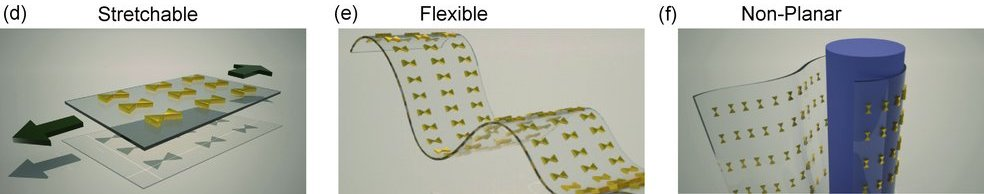
\includegraphics[width=\columnwidth]{01flexibility.jpg}
\caption{Charactersitics of flexible substrates (Source \cite{paper}): d) shows the application of mechanical strain, which can be used to tune the optical properties. e) and f) demonstrate how structures on the flexible films can be transferred and wrapped around nonplanar surfaces.}
\label{fig:flexibility}
\end{center}
\end{figure}

	Another field, where research on flexibility is conducted and where more progress has been achieved so far is flexible electronics. For example, paper-like display devices and biointegrated electronics for in vivo brain monitoring have already been created. 
	
	In comparison, progress with flexible photonics was very limited so far because of difficult fabrication with traditional techniques, the small feature dimensions below 100nm, the mechanically compliant surfaces and the fact, that conventional operation temperature and chemicals are not compatible with the new substrates. The existing methods for patterning flexible substrates mostly use soft lithography like replica molding or decal transfer lithography.

\begin{figure}[hbt!]
\begin{center}
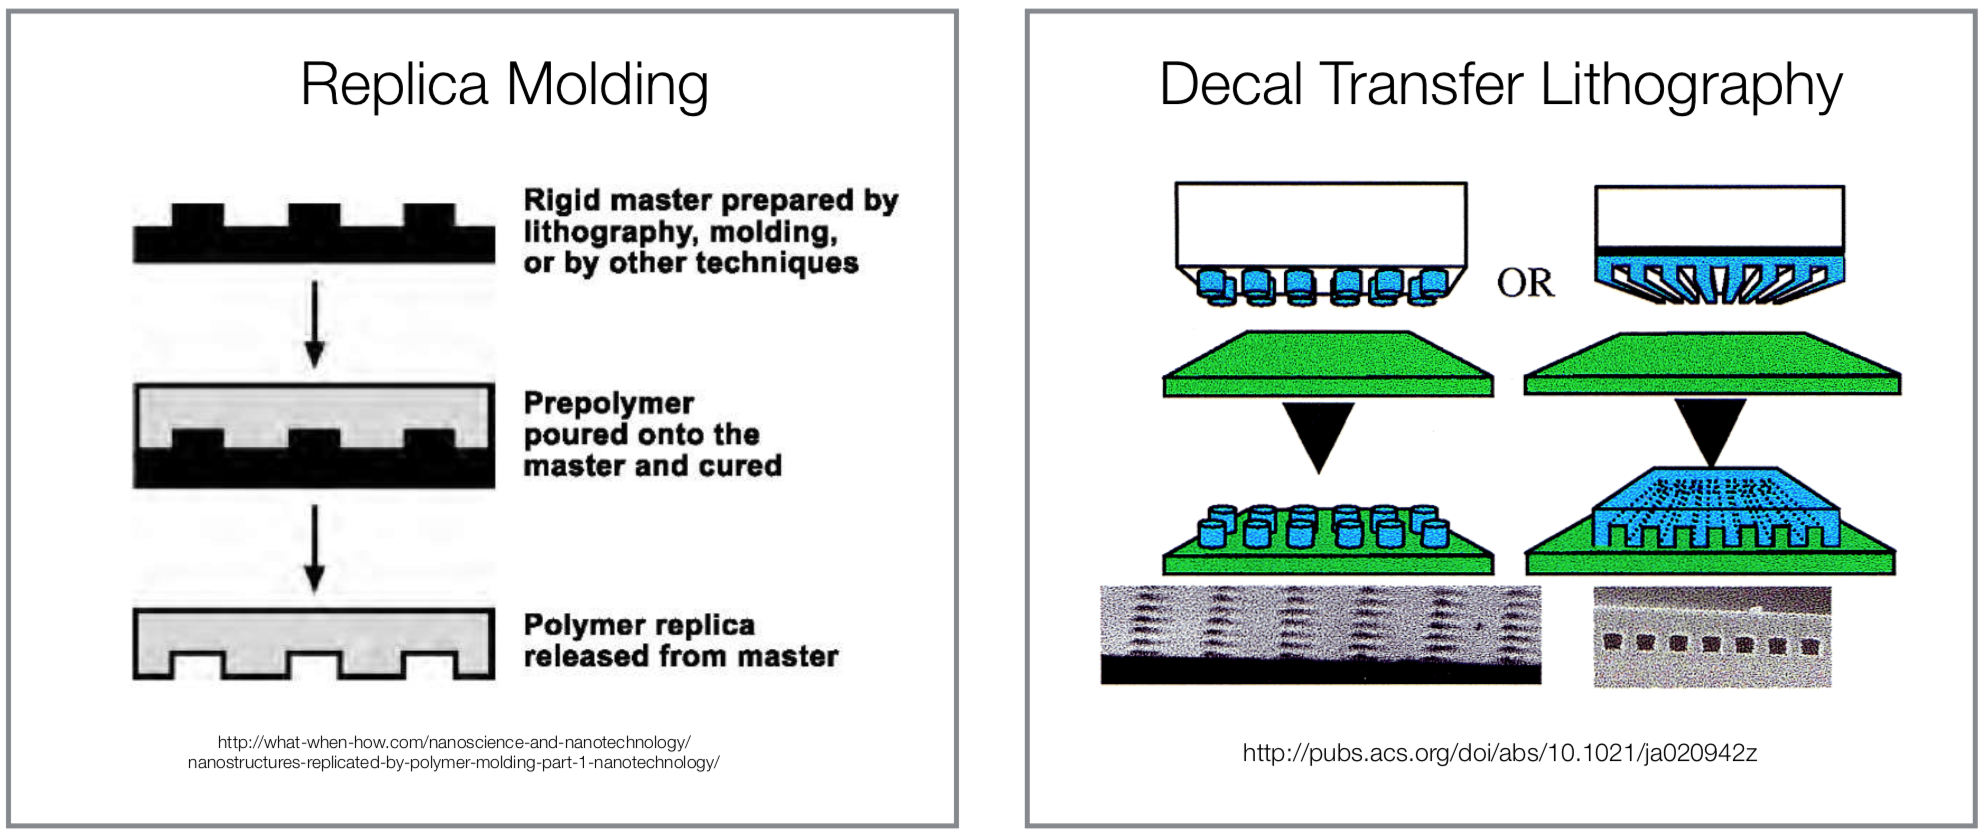
\includegraphics[width=\columnwidth]{02softlitho.png}
\caption{Common soft lithography techniques (Sources \cite{replica} and \cite{decal})}
\label{fig:soft-litho}
\end{center}
\end{figure}	

For replica molding, a rigid master has to be prepared by techniques as lithography, then the polymer is poured onto the master and cured. Decal transfer lithography uses a carrier to bring the structures onto the flexible substrate. The problem with these conventional techniques is their limited versatility, wich is because they are either complex and require multiple fabrication steps, which degrades the resolution or because only special materials can be used for patterning. 

The solution for good results with flexible substrates is a new fabrication technique, nanostencil lithography, which will be explained in the following and was used to obtain all the results in the discussed paper \cite{paper}.


\section{Main Part}
First, we introduce the materials used as flexible substrates, second, the new nanostencil lithography technique will be explained and associated problems and improvements will be discussed. Then the fabrication and characterisation of bow ties and antenna arrays will be presented. Lastly, new functionality through the flexibility is shown, namely stretching and nanopatterning. 

\subsection{Nano Stencil Lithography}	

\subsubsection{Materials used as flexible substrates}
To get a better feel for the flexible substrates, we introduce the different materials and their interesting applications supported by pictures from an internet search.

\begin{figure}[hbt!]
\begin{center}
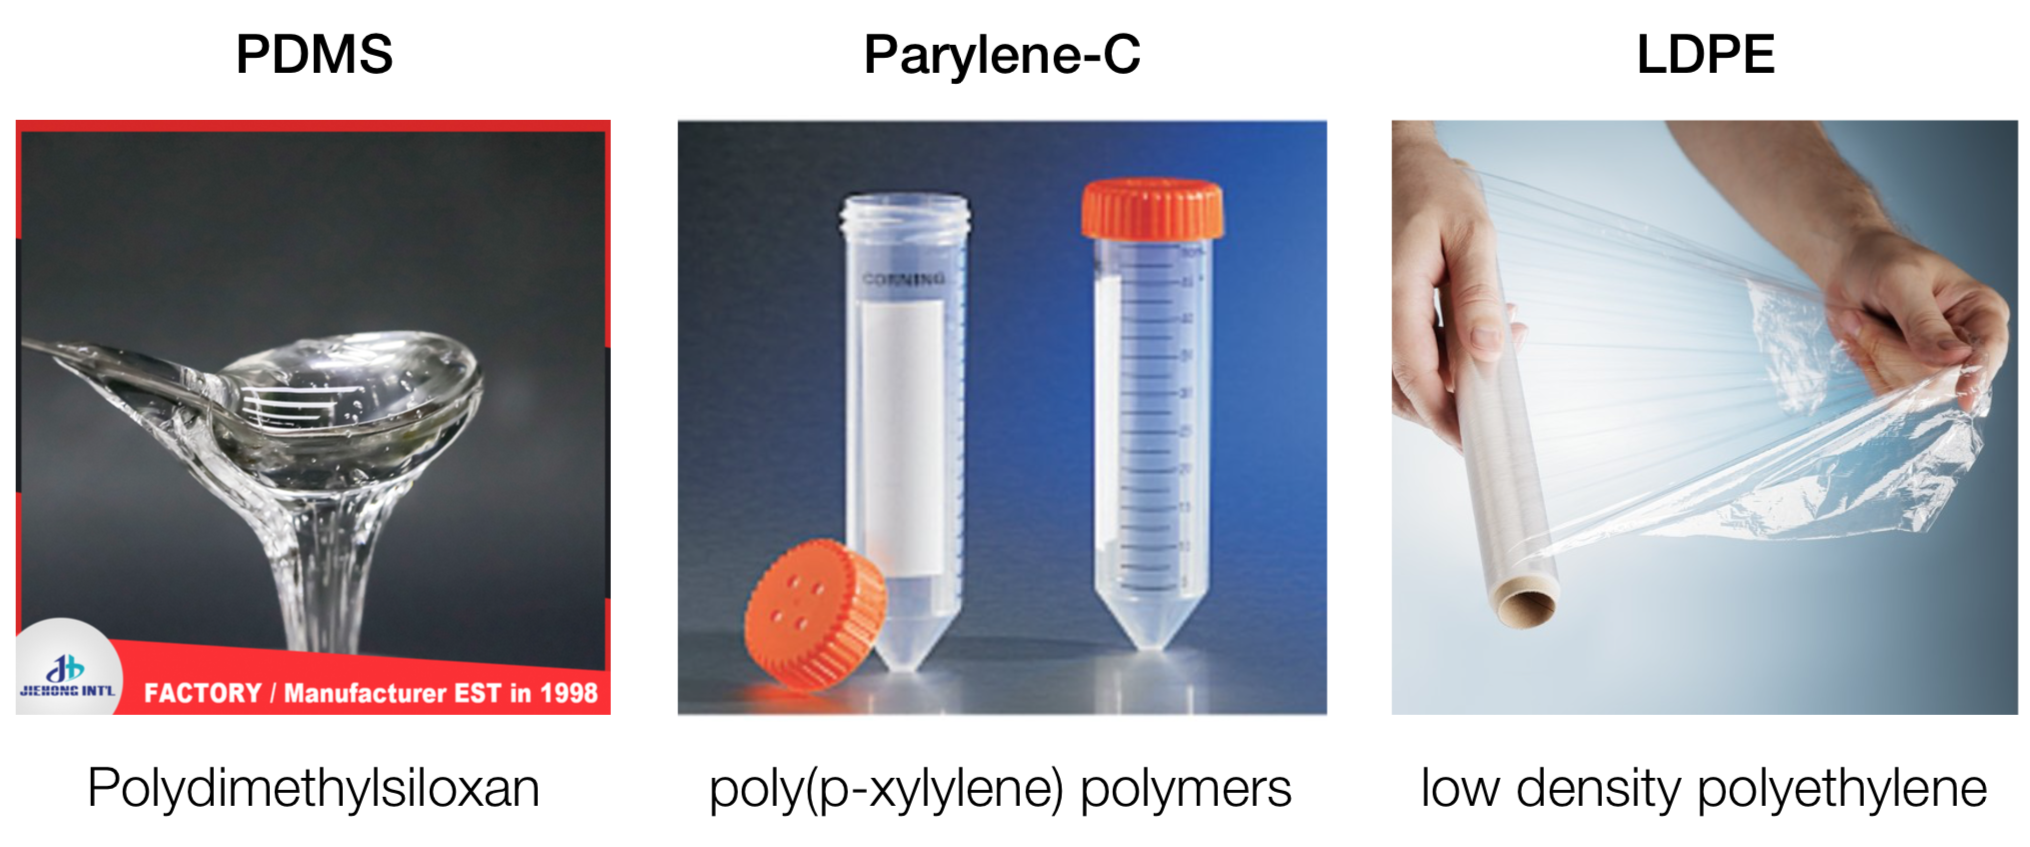
\includegraphics[width=\columnwidth]{03substrates.png}
\caption{Flexible polymer substrates (Sources \cite{PDMS}, \cite{Parylene-C}, \cite{LDPE})}
\label{fig:substrates}
\end{center}
\end{figure}

PDMS is a thick silicon oil, wich can be spin coated and cured to give a flexible substrate. It is also used across industries, for example in shampoos. The thickness of the PDMS used substrate is 100 $\mu$m. The second material is Parylene-C, often used as hydrophobic and chemically resistant coating in tubes and medical accessory. It is also of use in electronics, because a thin layer of the material makes electronics water-resistant. For our purposes, a thickness of 5 $\mu$m will be used. As the title of the paper indicates, an unconventional substrate was tested, which is LDPE (low density polyethylene) in the form of food storage rolls available in convenience stores with a thickness of 13 $\mu$m.

	
\subsubsection{The NSL process and its properties}
In nanostencil lithography, a stencil is placed on the substrate, then material (e.g. gold) is deposited to create the structures. When the stencil is removed, only the structures stay on the substrate. Afterwards, the stencil can be cleaned and reused.

\begin{figure}[hbt!]
\begin{center}
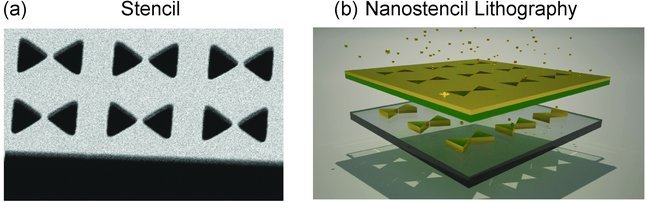
\includegraphics[width=\columnwidth]{04nsl.jpg}
\caption{Nanostencil Lithography (Source \cite{paper})}
\label{fig:nsl}
\end{center}
\end{figure}

The stencil itself can be fabricated from a silicon nitride (SiN$_x$) membrane, where the apertures can be created with electron beam lithography (EBL) and dry etching. This way, the stencil is mechanically robust, easy to carry and clean for multiple usages. With these properties, the new nanostencil lithography technique offers high resolution, requires only a single fabrication step and is applicable on a wide range of flexible substrates.

\subsubsection{NSL problems} 
As the nanostencil is rigid, a gap between the stencil and the substrate can arise when the stencil is placed on an uneven surface or if there is bending or curving of the stencil membrane itself. This leads to the problem of deposition of material underneath the stencil membrane. 

\begin{figure}[hbt!]
\begin{center}
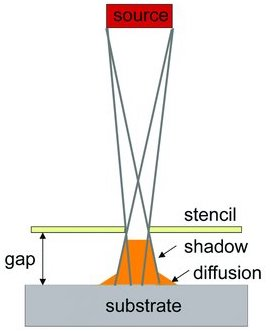
\includegraphics[width=0.8\columnwidth]{05gap.jpg}
\caption{Problems associated with substrate-mask-gap (Source \cite{paper})}
\label{fig:gap}
\end{center}
\end{figure}

There are three consequences resulting from the gap between substrate and mask, which are illustrated in Figure \ref{fig:gap}: 

Problem 1 - shadow: dimensions are larger than apertures \\Problem 2 - diffusion: a halo layer around the structure appears \\Problem 3 - cone shape: the vertical profile is tapered

\subsubsection{NSL improvements} 
These problems can be overcome when the nanostencil lithography is performed on a polymeric substrate with an elastic adhesive surface, for example PDMS. The hydrophobic surface, low surface energy and elasticity of PDMS promotes weak bonding with the stencil mask and eliminates the gap. Without the gap, the problems vanish.

\begin{figure}[hbt!]
\begin{center}
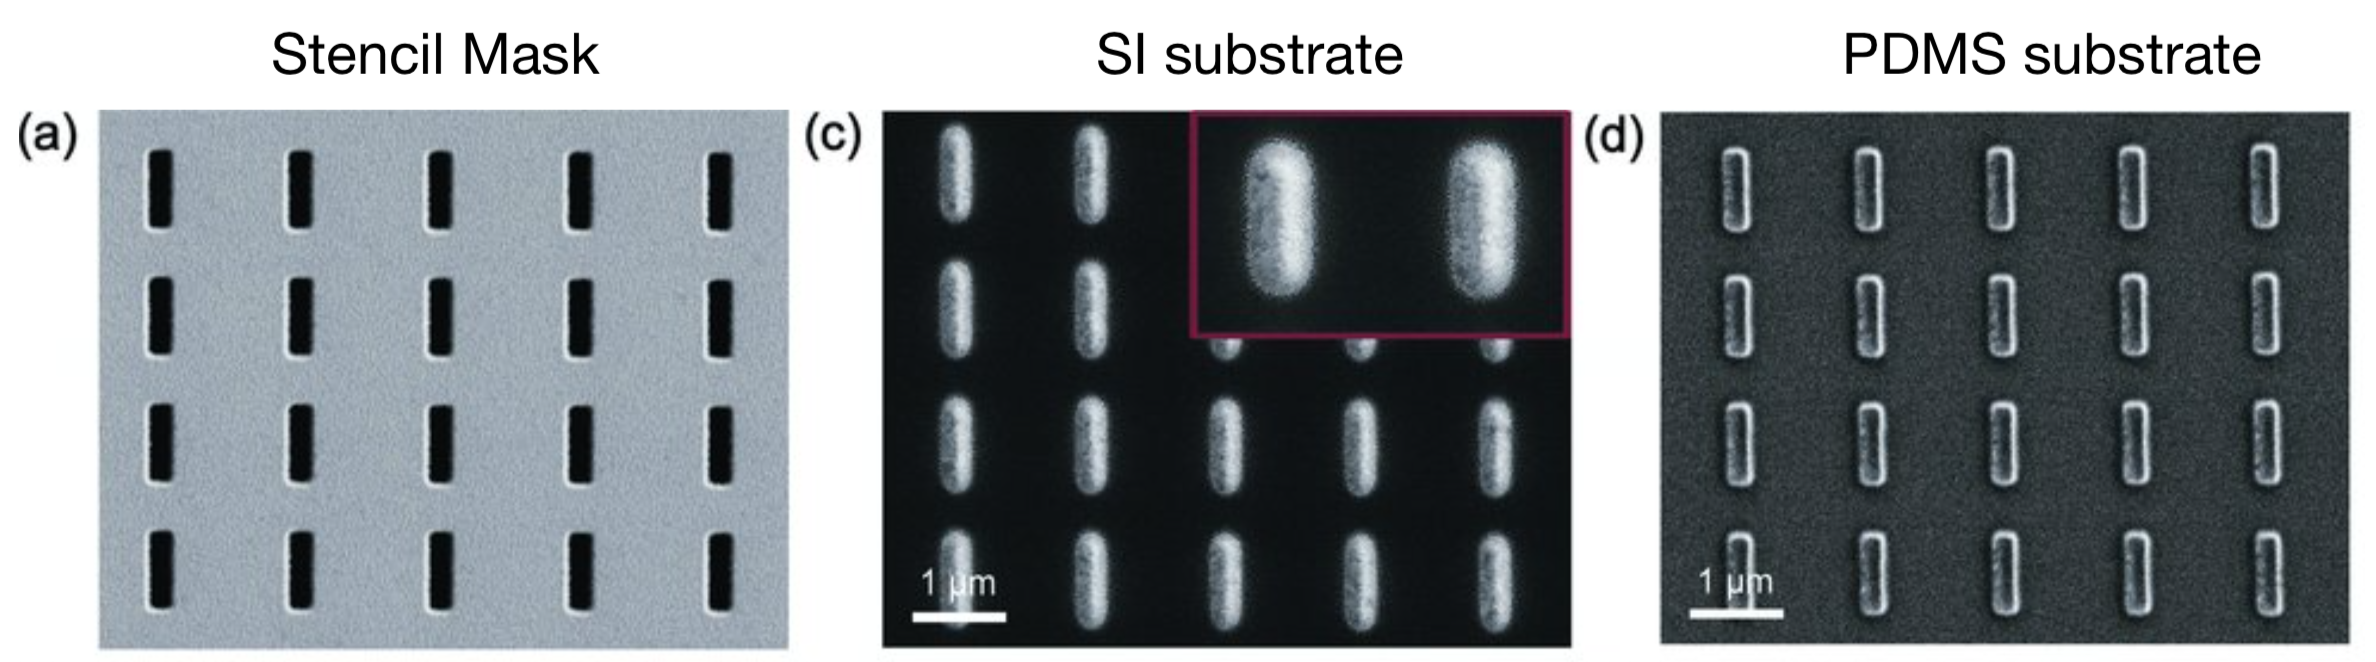
\includegraphics[width=\columnwidth]{06nogap.png}
\caption{SI substrate vs PDMS substrate (Source \cite{paper}): a) shows a SEM image of the stencil mask, apertures 940nm by 245nm in size, periodicity 1.5 $\mu$m. While we can observe the halo effect with SI substrate in c), the results are good when using PDMS substrate d)}
\label{fig:nogap}
\end{center}
\end{figure}

Especially the profiles generated by atomic force microscopy show the improvement through PDMS substrate. While we find a cone shape and a hight of only 120nm (150nm were deposited) with Si-substrate, the profile with PDMS is sharp, well defined and the height much closer to the thickness of deposited material.

\begin{figure}[hbt!]
\begin{center}
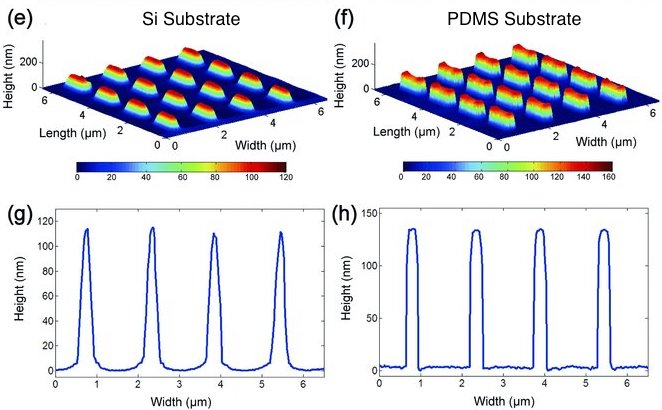
\includegraphics[width=\columnwidth]{07profiles.jpg}
\caption{AFM profiles on SI and PDMS (Source \cite{paper}) Structures on Si have a tapered wall profile with less height compared to the structures on PDMS.}
\label{fig:profiles}
\end{center}
\end{figure}

\subsubsection{NSL repeatability}
A key feature of nanostencil lithography is the repeated fabrication with the same stencil. This feature was tested using three identical masks and three repetitions, the masks were cleaned using gold etchant. On the rigid silicon substrate, the standard deviation was 113nm, whereas on the flexible PDMS, the fabricated dimensions have an average accuracy of 9nm and a standard deviation of 6.22nm, which is near the AFM resolution limit of 4nm. These results show that with polymeric interfaces, significant improvement of resolution and high repeatability is achieved.


\subsection{Bow Ties and Antenna Arrays}
For a better understanding of the performance of nanostencil lithography on flexible substrates, two structures are fabricated and optically characterised.

\begin{figure}[hbt!]
\begin{center}
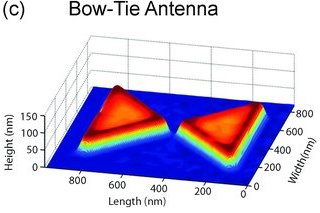
\includegraphics[width=0.9\columnwidth]{08bowtie.jpg}
\caption{AFM image of a Bow-Tie Antenna (Source \cite{paper})}
\label{fig:bowtie}
\end{center}
\end{figure}

\subsubsection{Bow Ties}
Bow Ties show novel electromagnetic responses induced by small gaps and asymmetries. While sharp edges and small gaps (less than 100nm) are difficult with nanostencil lithography on conventional substrates, on PDMS high quality bow ties with sharp edges have been achieved. The dimensions in figure \ref{fig:bowties} are: sidelength 645nm, thickness 50nm, interparticle distances 25nm to 45nm.

\begin{figure}[hbt!]
\begin{center}
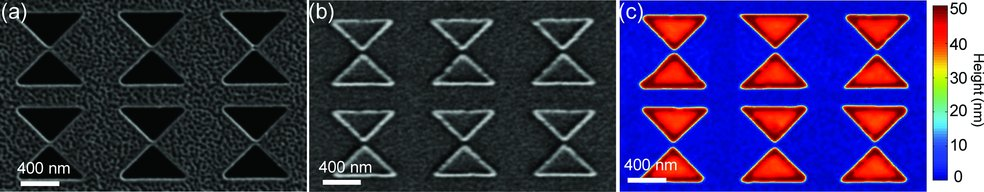
\includegraphics[width=\columnwidth]{09bowties.jpg}
\caption{Bow-Tie Antennas (Source \cite{paper}) Left picture shows a SEM image of a bow-tie-stencil mask, triangles with side lengths of 645nm and separation of about 55nm. Middle SEM picture shows bow ties on PDMS, accuracy down to 10nm. Right picture shows AFM images of bow-ties}
\label{fig:bowties}
\end{center}
\end{figure}

For the measurement, bow ties with three interparticle distances on PDMS are illuminated with visible polarized light. Both experimental results and calculation via a Hybridization Model show that a decreasing gap leads to a redshift of the resonance wavelength. Hence fine-tuning of the resonance wavelengths is possible.

\begin{figure}[hbt!]
\begin{center}
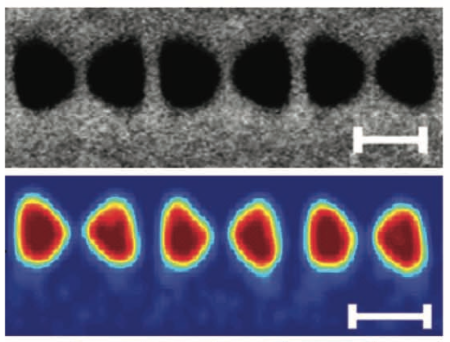
\includegraphics[width=0.4\columnwidth]{092bowties.png}
\caption{Bow-Tie Antennas (Source \cite{paper}) for the following optical characterisation in fig. \ref{fig:bowtie-resonance}. Scalebar is 200nm. Upper SEM image shows stencil, separation 25nm, sidelength 100nm. Bow ties in AFM picture below have 35nm distance and 85nm side lengths.}
\label{fig:bowties2}
\end{center}
\end{figure}

\begin{figure}[hbt!]
\begin{center}
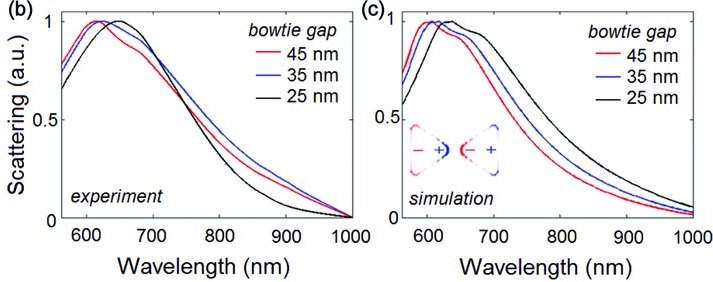
\includegraphics[width=\columnwidth]{10bowtie-resonance.jpg}
\caption{Bow-Ties: Optical Characterization (Source \cite{paper}) Left: Experimental measurements of optical spectrum (bow tie side length 85nm, distance 25nm to 45nm. Visible is red-shift of resonance with decreasing bow-tie gap. Right: Numerical calculations with dimensions as fabricated confirm experimentally obtained resonances and shifts.}
\label{fig:bowtie-resonance}
\end{center}
\end{figure}

\subsubsection{Antenna Arrays}
The second investigated structure was an array of golden rods. The goal here is to create enhanced near-field intensities at nano-tips, wich are amplified through collective excitations. 

\begin{figure}[hbt!]
\begin{center}
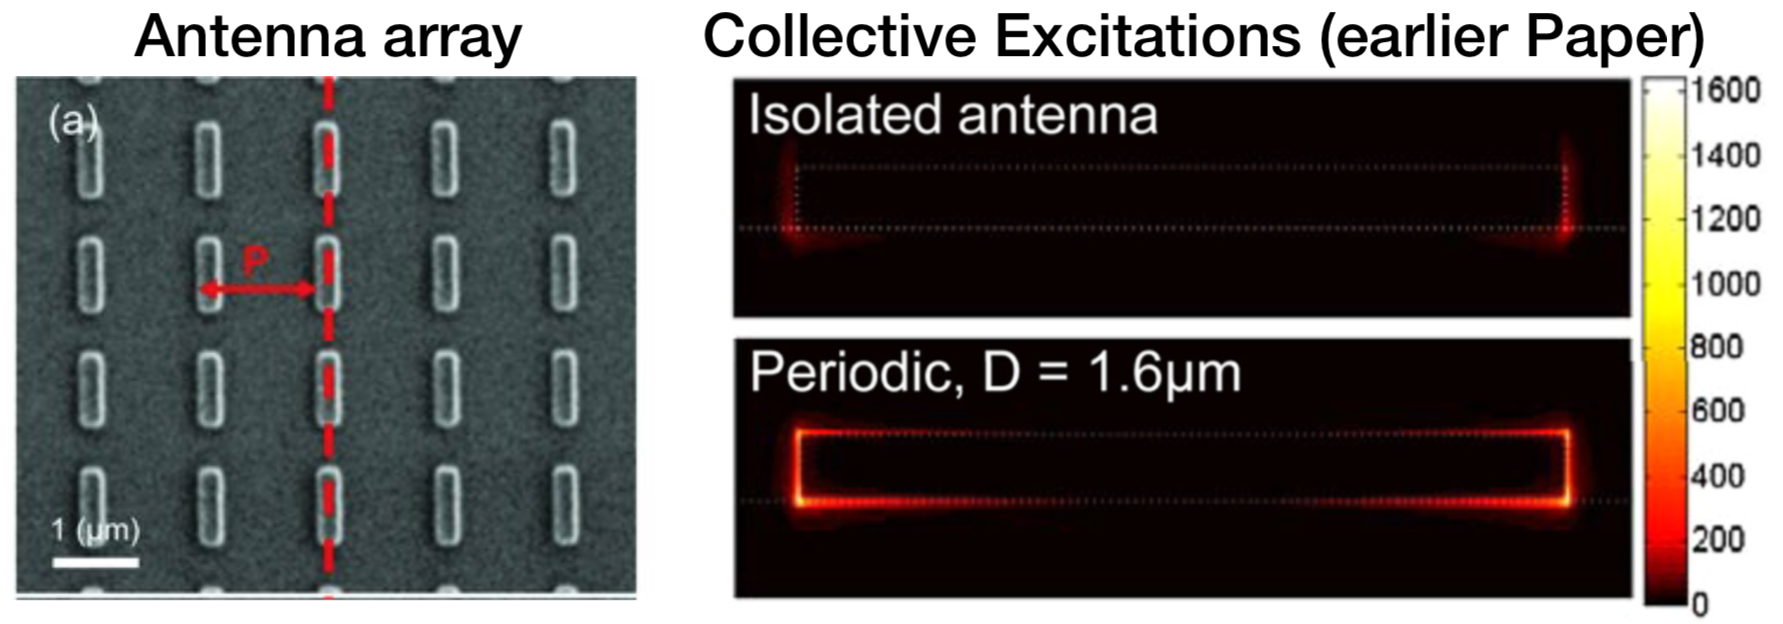
\includegraphics[width=\columnwidth]{11collective.png}
\caption{Collective Excitations \cite{collective-paper} of Antenna arrays: Collective resonances in periodic arrangements of nanoantennas can give rise to nearly an order of magnitude larger near-field intensity enhancements compared with the isolated antenna. Shown are Cross-sections of the intensity distribution taken through the edge of the rod are shown for periodic (d   1.6 $\mu$m) and isolated antenna.}
\label{fig:collective}
\end{center}
\end{figure}

There are two parameters that can be tuned which correspond to sizes of the array. The first is the resonance of the localized surface plasmon (LSP) which can be tuned by the rod length. The second are the photonic resonances of the array, the grating orders, to be tuned by the periodicity of the array. The transmission spectra in fig.\ref{fig:transmission} are obtained by varying one parameter while holding the other constant. We observe, that the nanorods on parylene-C follow the modified antenna theory: Increasing rod length and periodicity result in redshift of the resonance wavelength.

\begin{figure}[hbt!]
\begin{center}
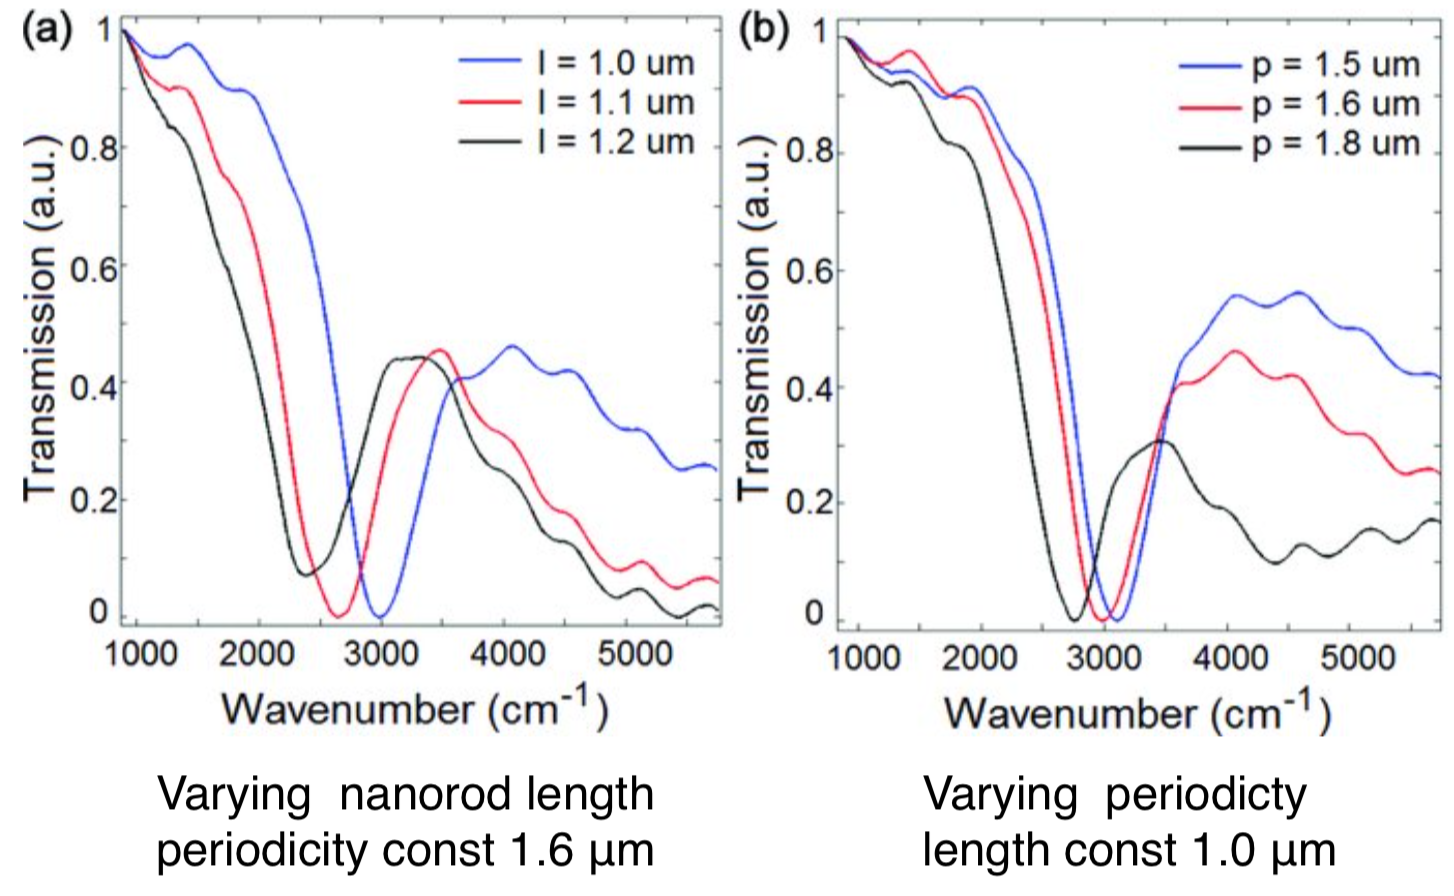
\includegraphics[width=\columnwidth]{12transmission.png}
\caption{Transmission spectra of gold nanorod antenna arrays on 5$\mu$m thick parylene-C (Source \cite{paper}). With increasing antenna length, red-shift of resonance occurs.}
\label{fig:transmission}
\end{center}
\end{figure} 

\subsection{Novel use of the substrate flexibility}
\subsubsection{Substrate stretching}
As seen with the Antenna Arrays, enlarging the periodicity of antenna arrays leads to a redshift of the resonance wavelength. The question now is, whether we can create the same effect not by two different structures but by enlarging the periodicity through stretching the flexible substrate and thus actively tuning the optical response. Investigation of gold nanorods on a 1mm thick PDMS substrate show, that mechanical stretching of PDMS in one direction leads to homogeneous periodicity increase (decrease) along the direction parallel (perpendicular) to the force. The periodicity enlarged from 1.51$\mu$m to 1.83$\mu$m. Moreover, when the applied tension is released, the substrate and nanorods return back to the initial position, the nanorods are not damaged and perfectly intact with the substrate. Thus, stretching only changes the periodicity but not the particle dimensions. 

\begin{figure}[hbt!]
\begin{center}
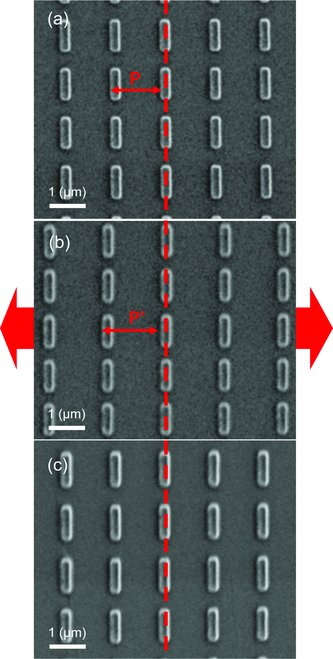
\includegraphics[width=0.65\columnwidth]{13stretch.jpg}
\caption{Stretching antenna array on PDMS (Source \cite{paper}): three SEM images are shown, rods with 945nm times 240nm, periodicity 1.515$\mu$m on PDMS. a) initial positions, b) application of force, c) force removed, rods return to initial position without being damaged.}
\label{fig:stretch}
\end{center}
\end{figure} 

The optical measurement shows that the stretch leads to the desired redshift of resonance wavelength and agrees with the calculation through finite difference time domain method (FDTD). These results show, that we can actively tune the resonance wavelenghts without damaging the device, which is a new material characteristic of flexible substrates.

% This is how you define a table: the [!hbt] means that LaTeX is forced (by the !) to place the table exactly here (by h), or if that doesnt work because of a pagebreak or so, it tries to place the table to the bottom of the page (by b) or the top (by t).
	\begin{table}[!hbt]
		% Center the table
		\begin{center}
		% Title of the table
		\caption{Stretch Parameters (fig \ref{fig:stretch-response})}
		\label{tab:simParameters}
		% Table itself: here we have two columns which are centered and have lines to the left, right and in the middle: |c|c|
		\begin{tabular}{|c|c|c|}
			% To create a horizontal line, type \hline
			\hline
			% To end a column type &
			% For a linebreak type \\
			Parameter & Left & Right\\
			\hline
			Redshift & 160 nm & 230 nm\\
			\hline
			P Enlargment & 5 \% & 16 \%\\
			\hline
			Length & 1200 nm & 900 nm\\
			\hline
			Periodicity & 1.5 $\mu$m & 1.8 $\mu$m\\
			\hline
		\end{tabular}
		\end{center}
	\end{table}

\begin{figure}[hbt!]
\begin{center}
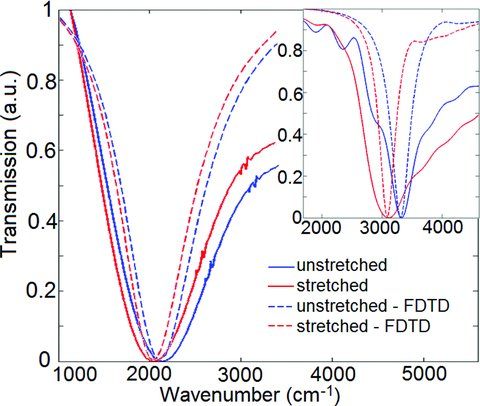
\includegraphics[width=\columnwidth]{14stretch-response.jpg}
\caption{Optical response to stretch (Source \cite{paper}) Measured and calculated (dashed) transmission spectra of nanorods (1.5$\mu$m periodicity, 1200nm length, on 13$\mu$m thick LDPE film. Inset: LDPE with 900nm gold rods. Blue curves: before stretching, red curves: after stretching}
\label{fig:stretch-response}
\end{center}
\end{figure} 

\subsubsection{Direct nanopatterning}
Nanopatterning means bringing nanostructures onto a surface via the substrate. In most cases, this is challenging or not possible with existing technologies as they are inherently 2D. Novel flexible substrates offer a three-step solution: First, the structures can be generated on a flexible 2D-film with nanostencil lithography. Second, the film can be used as carrier to transfer the structures to the curved surface. Third, the carrier polymer can be removed by selective etching, if needed.

This process works and was demonstrated on optical fibers: Circular gold particles (2 $\mu$m were patterned onto a bare fiber optic cable with 300 $\mu$m using a paylene-C film as carrier. Looking forward, the same technique could be one day used to pattern nanostructures onto veins in the human body and thus creating truly integrated sensor systems. 

\begin{figure}[hbt!]
\begin{center}
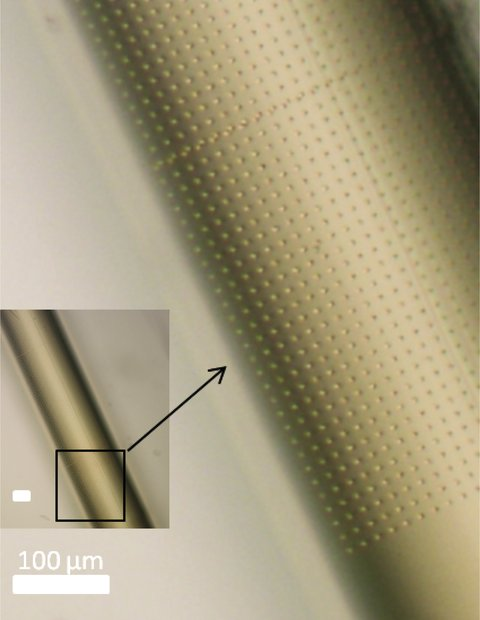
\includegraphics[width=0.8\columnwidth]{15patterning.jpg}
\caption{Direct nanopatterning on fibre optic cable (Source \cite{paper}) Flexible 10 $\mu$m thick parylene-C film patterned with circular gold particles of 2 $\mu$m diameter and 10 $\mu$m periodicity}
\label{fig:patterning}
\end{center}
\end{figure} 


\section{Summary}
The new results show, that flexible substrates can be patterned with high precision and offer new possibilities. 

In particular, nano stencil lithography enables single-step, high-throughput, high-resolution, large-area fabrication. The resolution limit is improved by using polymeric substrates with adhesive surface. The new technique can even replicate the resolution of the industry gold-standard EBL down to 10nm accuracy. 

The bow tie fabrication showed, that sub-50nm gap distance and sub-100nm side lengths is possible with nanostencil lithography on flexible substrates. Furthermore, precise control over the interparticle distance has been achieved.

With nano antenna arrays, plasmonic resonance have been studied. Key result was the active tuning of red-shifting the resonance wavelength through stretching the flexible substrates.

Lastly, nanopatterning of curved surfaces was demonstrated by wrapping nano-patterned flexible substrates around a nonplanar surface. 


\section{Discussion}
The results of the paper "Flexible Plasmonics on Unconventional and Nonplanar Substrates" by Serap Aksu et al. may seem intriguing and they are in fact quite impressive. Nevertheless, we should also take a critical look on the work. 

Considering the Nanostencil Lithography Technique NSL, we observe, that the accuracy of features degrades when small sizes are approached. For example, figure \ref{fig:bowties2} should actually represent bow-ties, but the resulting structures lose their sharpness and look circular. This effect is already seen in the mask, which is created using electron beam lithography.  Here, a new way has to be found to create sharper features. 

The authors of the paper also claim, that NSL enables high-throughput fabrication and argued, that they could use the same stencil three times. For industrial applications, the repeatability has to be tested more thoroughly. There is no data on how many repetitions are possible or whether the quality degrades after three cycles or more.

Using the adhesive surface of PDMS to eliminate the gap between surface and stencil is a nice trick which can be used in other circumstances as well. 

What's also not clear from the shown results is whether the stencils are able to create homogeneous structures on the whole surface or if some other degrading effects appear in some regions, which is important to know for large-scale fabrication.

The Bow-Tie antennas showed a nice optical response. In fact, the agreement of experiment to simulation in the optical characterization is so good, that we'd have to ask if this is repeatable or if only a good picture was picked.

When the nanorod arrays were discussed, the stretching of the substrate was done only once. Here it would be of value to see a time-series of the response to stretching and examine the changing parameters. One could test how for how long stretching is possible and if the effect changes over time. In the paper, there was mentioned that structures are not damaged when they return, but this was determined only optically. An important measurement would be to determine the force needed to peel off the structures from the elastic substrate, for example with an AFM-setup. Then we'd know better whether the structures stick to the substrate, even after multiple stretches.

The direct nanopatterning is also a nice last result. Here the authors of the paper took an easy choice in patterning the cable, which is bent only in one direction. It would be interesting to see wether the patterning also works on more difficult topologies. 



\section{Conclusion}
Overall, the paper shows impressive results and points towards an interesting research direction. Especially active tuning of resonance frequencies is a great finding.
Having knowledge of the new achievements gives us the opportunity to think beyond the currently possible and use the newly won characteristics of flexible substrates for our own purposes. 


% You can cite a book or paper by using \cite{reference}.
% The references will be defined at the end of this .tex file in the bibliography
% (example: ``... as shown in \cite{HOP96}, ...'').
% You can reference tables and figure by using the \ref{label} command. Each table and figure needs to have a UNIQUE label.
% Figures and tables should be labeled and numbered, such as in Table~\ref{tab:simParameters} and Fig.~\ref{fig:tf_plot}.
% If you have questions about how to write mathematical formulas in LaTeX, please read a LaTeX book or the 'Not So Short Introduction to LaTeX': tobi.oetiker.ch/lshort/lshort.pdf


% Now we need a bibliography:
\begin{thebibliography}{5}

\bibitem{paper} % Main resource
Serap Aksu, Min Huang et al.: Flexible Plasmonics on Unconventional and Nonplanar Substrates (Main resource for this report)

\bibitem{replica}
Replica Molding Image: http://what-when-how.com/nanoscience-and-nanotechnology/nanostructures-replicated-by-polymer-molding-part-1-nanotechnology/

\bibitem{decal}
Decal Transfer Lithography Image: http://pubs.acs.org/doi/abs/10.1021/ja020942z

\bibitem{PDMS}
PDMS Image: \url{https://www.alibaba.com/product-detail/PDMS-polydimethylsiloxane-201methyl-siliconeoil_60719292898.htmlspm=a2700.7724838.2017005.1.9c5d76dsCYXRc}

\bibitem{Parylene-C}
Parylene-C Image: \url{https://www.fishersci.ch/ch/de/ products/I9C8L7UU/centrifuge-tubes.html}

\bibitem{LDPE}
LDPE Image: \url{https://deavita.com/haushalt/tipps-tricks-h aushalt-frischhaltefolie-ideen.html}

\bibitem{collective-paper}
Ronen Adato et al: Ultra-sensitive vibrational spectroscopy of protein monolayers with plasmonic nanoantenna arrays 


\end{thebibliography}

% Your document ends here!
\end{document}